\documentclass[fullpage,12pt,fleqn]{article}
\usepackage{graphicx}
\usepackage{verbatim}
%\usepackage{biblatex}
%\usepackage{natbib}
%\usepackage{natbib}
\usepackage[square,sort,comma,numbers]{natbib}
\bibliographystyle{unsrtnat}
%\input{commands}
%\input{bibstuff}

\newcommand{\RNold}[1]{\underline{r}_{#1}}
\newcommand{\nCr}[2]{\left(\begin{array}{c} #1 \\ #2 \end{array}\right)}
\newcommand{\half}{\frac{1}{2}}

\title{Notes on the evaluation of coupling-coefficients and Hamiltonian matrix-elements using determinants and configuration state functions.}

\author{Robert J. Harrison}

\date{}

\begin{document}
\maketitle

\clearpage

\tableofcontents

\clearpage

\section{Introduction}

For the purpose of evaluating matrix elements over a wide variety of
density operators, while grouping all possible spin functions for a
given orbital occupation and also having the ability to use either CSF
or determinants, I have adapted a full-CI program that I wrote while at
Argonne National Laboratory in 1986/7.  It has required some
modification for the present purposes and additional changes are
necessary, however, its internal structure is very simple and it
should be easy to extend, fast and correct!

These notes serve to describe the theory behind the code and the
coupling-coefficient generation and spin adaption used in the program.
The methodology is standard and draws very heavily upon Pauncz
\cite{pauncz,paunczsym}, Handy \cite{handyfci}, Knowles
\cite{knowleseai} and especially Duch
\cite{duchug,duchspinad,duchcouple,duchfci,duchsga}.  Graphs provide a
very simple, visually accessible and computationally useful
representation of many types of bases, espcially of ``complete-bases''
such as full-CI, CISD, or all possible spin functions for a given
open-shell occupation.  The graphical unitary group approach
\cite{paldusguga,shavittguga,shavittguga2} perhaps first demonstrated
the utility of this approach and it was applied in the symmetric group
approach by Duch et al \cite{duchsga}.  The program internally uses
graphical representations only for the lexical ordering of orbital and
spin occupations.  It does not use a graphical approach for the
evaluation of matrix elements.  There is no advantage to this for FCI
and the modern thinking seems to be that graphical approaches of the
1970's and 1980's are unecessarily complex (c.f., the marvellous
analysis of the MRSDCI algorithm by Saunders and van Lenthe
\cite{saunders}).

I don't think that I have done anything new here.  The notes are very
basic so that the program is usable even by someone unfamiliar with CI
methodology, or a graduate student.

\section{Determinant bases}

 For the present purpose we shall assume that all molecular orbitals
($\phi$) are real, orthonormal, and that spin orbitals ($\varphi$) are
constructed as a product of the spatial and spin components.  For
instance,
\begin{equation}
 \varphi_{i}(\RNold{1}) = \phi_i(\RNold{1}) \sigma_i(1)
\mbox{, $\sigma_i = \alpha$ or $\beta$}
\end{equation}
A determinantal electronic wavefunction ($\Phi$) is simply an
antisymmetrized product of spin orbitals:
\begin{eqnarray}
  \Phi & = & \left| \varphi_{1}(\RNold{1}) \varphi_{2}(\RNold{2}) \cdots
\varphi_{n}(\RNold{n}) \right | \\
       & = & {\cal A} \; \varphi_{1}(\RNold{1}) \varphi_{2}(\RNold{2}) \cdots
\varphi_{n}(\RNold{n}) \\
{\cal A} & = & \frac{1}{\sqrt{n!}} \sum_{P} (-1)^P P.
\end{eqnarray}
${\cal A}$ is the antisymmetrizer and the sum in its definition ranges
over all possible $n!$ permutations of the $n$ electrons.  When we
start evaluating matrix elements it will be important to note that the
permutations act on the electronic coordinates (space and spin) and
not on the labels of the orbitals.  

A determinant is fully specified by
\begin{itemize}
\item the occupation of each spin orbital, and
\item an order in which the spin orbitals are occupied.
\end{itemize}
Clearly changing the order of the spin orbitals can change the sign of
the determinant, and thus consistency is crucially important. 

One very common ordering, especially for full-CI programs
\cite{handyfci}, is to occupy all alpha spin orbitals before all beta spin
orbitals, and suborder by spatial orbital index within each group.
\begin{equation}
\underbrace{\phi_{1}(\RNold{1})\alpha(1) \cdots
\phi_{n_{\alpha}}(\RNold{n_{\alpha}})\alpha(n_{\alpha})}_{\mbox{Alpha orbitals}}
\underbrace{\phi_{n_{\alpha}+1}(\RNold{n_{\alpha}+1})\beta(n_{\alpha}+1) \cdots 
\phi_{n}(\RNold{n})\beta_{n}(n)}_{\mbox{Beta orbitals}}
\end{equation}
The alpha or beta occupations are often referred to as strings.  This
separate treatment of each spin leads to a natural ordering of the
determinants, and makes the evaluation of matrix elements in a
determinant basis very straightforward.  However, it is is not
convenient for applications which need to manipulate all functions
with a given occupation of spatial orbtials (since these determinants
will be scattered throughout the CI vector) and should a fully
spin-adpated implementation be required very little code can be
reused.  

\label{standardorder}

The graphical representations used below unite determinant and
spin-adapted approaches, and also preserve the simplicity of the
evaluation of matrix elements over determinants while providing the
option of using fully spin-adpated bases.  For these reasons, let us
choose an order with
\begin{itemize}
\item all doubly occupied orbitals first (i.e., on the left) ordered
by increasing orbital index, and within each pair have the alpha
spin-orbital precede the beta spin-orbital, and
\item all singly occupied orbitals next, ordered by increasing orbital
index.
\end{itemize}
\begin{equation}
\underbrace{\phi_{1}(\RNold{1})\alpha(1)\phi_{1}(\RNold{2})\beta(2) \cdots
\phi_{d}(\RNold{2d})\beta(2d)}_{\mbox{doubly occupied}}
\underbrace{\phi_{d+1}(\RNold{2d+1})\sigma_{d+1}(2d+1) \cdots 
\phi_{d+s}(\RNold{n})\sigma_{n}(2d+s)}_{\mbox{singly occupied}}
\end{equation}
with $d$ doubly-occupied orbitals, and $s$ singly-occupied (or
open-shell) orbitals.  
It is more convenient if we group the spatial and spin
functions separately,
\begin{eqnarray}
\Phi & = & {\cal A} \; \left[
\left(\phi_{1}(\RNold{1})\phi_{1}(\RNold{2}) \cdots \phi_{d}(\RNold{2d})
\phi_{d+1}(\RNold{2d+1}) \cdots \phi_{d+s}(\RNold{n}) \right)\right. \\
 & & \left.\left(\alpha(1)\beta(2) \cdots \beta(2d) \sigma_{d+1}(2d+1) \cdots 
\sigma_{n}(2d+s)\right)\right]
\end{eqnarray}
This makes it clear that the {\em spin function depends only upon the
open shell orbitals}.  This is because each doubly occupied orbital
always has an alpha and a beta spin function in the specified order
and thus a doubly occupied orbital may be placed anywhere since the
two functions will always be moved together (i.e, it will be an even
permutation) and therefore the sign of the determinant will be
unchanged.  It is only ever necessary to consider the closed-shell
orbitals explicitly when computing matrix elements that involve these
indices, and then it suffices to consider any closed-shell pairs as
simply being two more open shells which happen to be numbered before
the `true' open shells.

It is also clear that the spatial functions (in the first set of
parentheses) and the spin functions may be managed separately.  I will
adopt uppercase Roman letters for spatial orbital occupation patterns
($|I\! >$) and the systematic construction of these is discussed below
in Section \ref{orbitalgraph}.  The $\mu$'th determinantal or
primitive spin function for $s$ electrons and $S_z = m$ will be
denoted by $\theta^{(s)}_{m,\mu}$ (in the program the routines that
deal with primitive spin functions often begin with the letter `m'
because of the identification of $S_z = m$).  If the Hamiltonian is
spin-free we only need to use functions with one value of $S_z$ and
the choice $S_z=S$ minimizes the dimension of the expansion space.

How many of these primitive spin functions functions are there?  There
are $(\half s + m)$ alpha spin electrons and $(\half s -
m)$ beta spin electrons to be distributed in all possible ways amoung
$s$ orbitals.  Thus, the number of primitive spin functions
(determinants) with $s$ open shells with given quantum number
$S_z=m$ is
\begin{equation}
d(s,m) = \frac{s!}{(\half s + m)! (\half s - m)!}
\end{equation}
By a similar argument, the dimension of a determinant full-CI
(ignoring spatial symmetry) with $n$ electrons in M orbitals and
$S_z=m$ is
\begin{equation}
D(M,n,m) = \nCr{M}{\half n + m}\nCr{M}{\half n - m}
\end{equation}

Our determinant, corresponding to the I'th orbital occupation which
has $s$ open shells, and the $\mu$'th primitive spin function for
the $s$ unpaired electrons coupled with $S_z=m$ is then finally
written as
\begin{eqnarray}
  |I\mu\! > & = & {\cal A} \; |I\! > \Delta \theta^{(s)}_{m,\mu} , \\
  |I\! > & = & \phi_{1}(\RNold{1})\phi_{1}(\RNold{2}) \cdots \phi_{d}(\RNold{2d-1}\phi_{d}(\RNold{2d})
\phi_{d+1}(\RNold{2d+1}) \cdots \phi_{d+s}(\RNold{n}) \\
  \Delta & = &\alpha(1)\beta(2) \cdots \alpha(2d) \beta(2d) \\
  \theta^{(s)}_{m,\mu} & = & \sigma_{d+1}(2d+1) \cdots
\sigma_{n}(2d+s)
\end{eqnarray}
where all of the closed-shell spin functions have been grouped into
$\Delta$ which never really needs to be considered.

\section{Graphical representation of primitive spin functions}

In this section we consider how the primitive spin functions are
numbered.  We wish to find an ordering for all possible primitive spin
functions for $s$ unpaired electrons with $S_z = m$.  A graphical
representation is very helpful.  In Figure \ref{mgraph} the coupling
of the Z-component spin of each open-shell electron is represented
with a line.  An upward line indicates alpha spin and a downward line
indicates beta spin.  There are only two possible choices of spin, and
we arrange for the graph to begin at the origin and end at the desired
$S_z$ and number of electrons (in this case $S_z = 0$ and 8
electrons).  Thus, the number of walks from left to right (or vice
versa) on this graph is equal to the total number of determinants.

\begin{figure}[htbp]

\center

%\centerline{\psfig{figure=mspingraph.eps,angle=270}}
\includegraphics[angle=270]{mspingraph.eps}
\caption{\label{mgraph} Graph of the primitive spin functions for 8
open-shell electrons coupled to $S_z=0$.}
\end{figure}

How many walks are there?  Each node on the graph in Figure
\ref{mgraph} is labelled with its weight which is the number of
possible ways of arriving at that node.  The weight of a node is the
sum of the weights of the (one or two) nodes that connect to it, and
the weight of the first node is one.  

A walk on the graph is commonly represented with a plus sign
(\verb!+!) or number 1 for upward moves (alpha occupation) and a minus
sign (\verb!-!) or number 2 for downward moves (beta occupation).  To
number each walk on the graph we must adopt some ordering and we use
the standard lexical order which places all functions coming from node
$(s-1,S_z+\half )$ before those from $(s-1,S_z-\half )$.
Thus, if when walking the graph from right to left we always stay as
high as possible we shall generate the lowest numbered walk.  The
lexical ordering for all walks in Figure \ref{mgraph} is given in
Table \ref{mwalks}.

\begin{table}[htbp]

\center

\begin{tabular}{lc|lc|lc}
 Index & Walk & Index & Walk & Index & Walk \\ \hline
 1 &  \verb!+ + + + - - - -! & 25  &  \verb!- - + + + - + -! & 49 &
\verb!+ - - + - + - +! \\
 2 &  \verb!+ + + - + - - -! & 26  &  \verb!+ + - - - + + -!    & 50 &
\verb!- + - + - + - +! \\
 3 &  \verb!+ + - + + - - -! & 27  &  \verb!+ - + - - + + -!    & 51 &
\verb!- - + + - + - +! \\
 4 &  \verb!+ - + + + - - -! & 28  &  \verb!- + + - - + + -!    & 52 &
\verb!+ - - - + + - +! \\
 5 &  \verb!- + + + + - - -! & 29  &  \verb!+ - - + - + + -!    & 53 &
\verb!- + - - + + - +! \\
 6 &  \verb!+ + + - - + - -! & 30  &  \verb!- + - + - + + -!    & 54 &
\verb!- - + - + + - +! \\
 7 &  \verb!+ + - + - + - -! & 31  &  \verb!- - + + - + + -!    & 55 &
\verb!- - - + + + - +! \\
 8 &  \verb!+ - + + - + - -! & 32  &  \verb!+ - - - + + + -!    & 56 &
\verb!+ + - - - - + +! \\
 9 &  \verb!- + + + - + - -! & 33  &  \verb!- + - - + + + -!    & 57 &
\verb!+ - + - - - + +! \\
10 &  \verb!+ + - - + + - -! & 34  &  \verb!- - + - + + + -!    & 58 &
\verb!- + + - - - + +! \\
11 &  \verb!+ - + - + + - -! & 35  &  \verb!- - - + + + + -!    & 59 &
\verb!+ - - + - - + +! \\
12 &  \verb!- + + - + + - -! & 36  &  \verb!+ + + - - - - +!    & 60 &
\verb!- + - + - - + +! \\
13 &  \verb!+ - - + + + - -! & 37  &  \verb!+ + - + - - - +!    & 61 &
\verb!- - + + - - + +! \\
14 &  \verb!- + - + + + - -! & 38  &  \verb!+ - + + - - - +!    & 62 &
\verb!+ - - - + - + +! \\
15 &  \verb!- - + + + + - -! & 39  &  \verb!- + + + - - - +!    & 63 &
\verb!- + - - + - + +! \\
16 &  \verb!+ + + - - - + -! & 40  &  \verb!+ + - - + - - +!    & 64 &
\verb!- - + - + - + +! \\
17 &  \verb!+ + - + - - + -! & 41  &  \verb!+ - + - + - - +!    & 65 &
\verb!- - - + + - + +! \\
18 &  \verb!+ - + + - - + -! & 42  &  \verb!- + + - + - - +!    & 66 &
\verb!+ - - - - + + +! \\
19 &  \verb!- + + + - - + -! & 43  &  \verb!+ - - + + - - +!    & 67 &
\verb!- + - - - + + +! \\
20 &  \verb!+ + - - + - + -= & 44  &  \verb!- + - + + - - +!    & 68 &
\verb!- - + - - + + +! \\
21 &  \verb!+ - + - + - + -= & 45  &  \verb!- - + + + - - +!    & 69 &
\verb!- - - + - + + +! \\
22 &  \verb!- + + - + - + -= & 46  &  \verb!+ + - - - + - +!    & 70 &
\verb!- - - - + + + +! \\
23 & \verb!+ - - + + - + -! & 47 & \verb!+ - + - - + - +! & \\
24 & \verb!- + - + + - + -! & 48 & \verb!- + + - - + - +! & \\ \hline
\end{tabular}

\caption{\label{mwalks} Lexical ordering of walks on the primtive spin
graph in Figure 1.}
\end{table}

Since we have all possible walks on the graph, then switching any two
orbitals will just generate another walk on the graph.

\section{Graphical representation of CSF bases}

Internally the program uses determinants, but provides the capability
of transforming to the Yamanouchi-Kotani \cite{kotani} genealogical
spin basis with conventional lexical ordering and numbering of
electrons (see Pauncz \cite{pauncz}).  This is the same as the
standard Young orthogonal representation which is also equivalent to
the Gelfand-Tsetlin basis of the unitary group approach.

The branching diagram (Figure \ref{sgraph}) depicts the construction
of a spin-adapted basis by the coupling of electronic spins.

\begin{figure}[htbp]

\center

%\centerline{\psfig{figure=spingraph.eps,angle=270}}
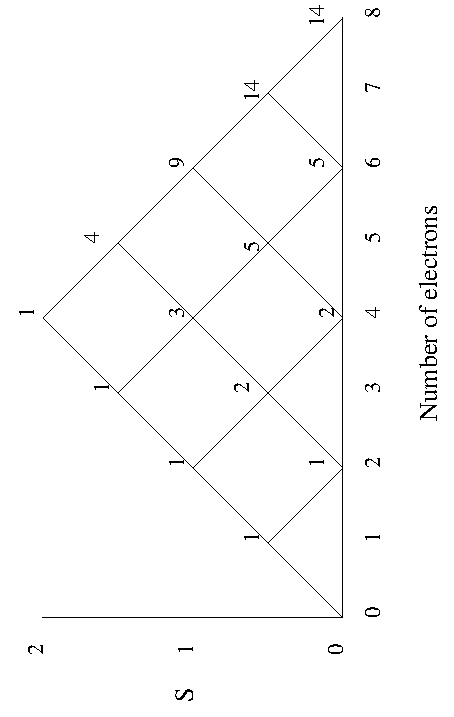
\includegraphics[angle=270]{spingraph.eps}
\caption{\label{sgraph} Branching-diagram or spin-coupling graph for 8
open-shell electrons coupled to a singlet.}
\end{figure}

 The spin-adpated basis is formed by using standard angular momentum
coupling methods.  Electrons are again added one at a time, but now
the total angular momentma are coupled, rather than just the $S_z$
component.  If some intermediate node has spin $S$, then adding an
alpha spin or beta spin electron will result in $S\pm\half $, but
we also have the constraint that $S \geq 0$.  Thus, all walks on the
spin-adpated graph must be above the horizontal axis, in contrast to
the graph for primitive spin functions ($-S \leq S_z \leq S$). It can
again be seen that walks on the graph represent all possible spin
functions and consideration of the spin-coupling shows that the
resulting basis is orthonormal.

How many spin adapted functions are there?  The determinants for given
$s$ and $S_z$ will form a complete basis for $S=S_z, S_z+1,\ldots$, and
thus
\begin{equation}
d(s,S) = f(s,S) + f(s,S+1) + \cdots + f(s,S_{max})
\end{equation}
Therefore, the number of spin-adpated functions for $s$ open-shell
electrons coupled to spin $S$ is
\begin{eqnarray}
f(s,S) & = & d(s,S) - d(s,S+1) \\
         & = & d(s,S) \frac{(2S + 1)}{(\half s + S + 1)} \\
         & = & \nCr{s+1}{\half s - S}\frac{(2S + 1)}{(s+1)}
\end{eqnarray}

The same argument may be invoked to demonstrate that the dimension
of a spin-adpated full-CI for $n$ electrons in $M$ orbitals for total
spin $S$, is
\begin{eqnarray}
 F(M,n,S) & = & D(M,n,S) - D(M,n,S+1) \\
          & = & D(M,n,S) \frac{(M+1)(2S+1)}{(\half n + S + 1)(M-\half n +S+1)}
\end{eqnarray}

The FCI program provides routines (see Section \ref{spinad1}) to
transform between the determinant and CSF spin bases for a given
open-shell occupation.  This follows the approach of Duch
\cite{duchspinad} but is readily constructed from the detailed
descriptions of the coupling in the books of Pauncz (e.g., see from
page 96 of \cite{paunczsym}).

\section{Graphical representation of orbital occupations}
\label{orbitalgraph}

Orbital occupations may be 0, 1, or 2 (empty, singly-, or
doubly-occupied) and are represented by walks on a 3-way graph
\cite{duchsga,duchfci}.  Since we are doing a full-CI we need all
possible walks.  Figure \ref{ograph} is an orbital graph for a full-CI
with 8-electrons in 8-orbitals without use of spatial symmetry.
Again, each node can be assigned a weight which is the sum of the
weights of the nodes that connect to it from above.  The weight of the
head (top node) is 1 and the weight of the tail (bottom node) is the
number of walks.


The lexical ordering of orbital walks is such that in traversing the
graph from bottom to top walks the rightmost arcs have lowest lexical
weight (the first and last twenty four walks on the graph in Figure
\ref{orbitalgraph} are given in Table \ref{owalks}).

\begin{figure}[htbp]

\center

%\centerline{\psfig{figure=orbitalgraph.eps,angle=270}}
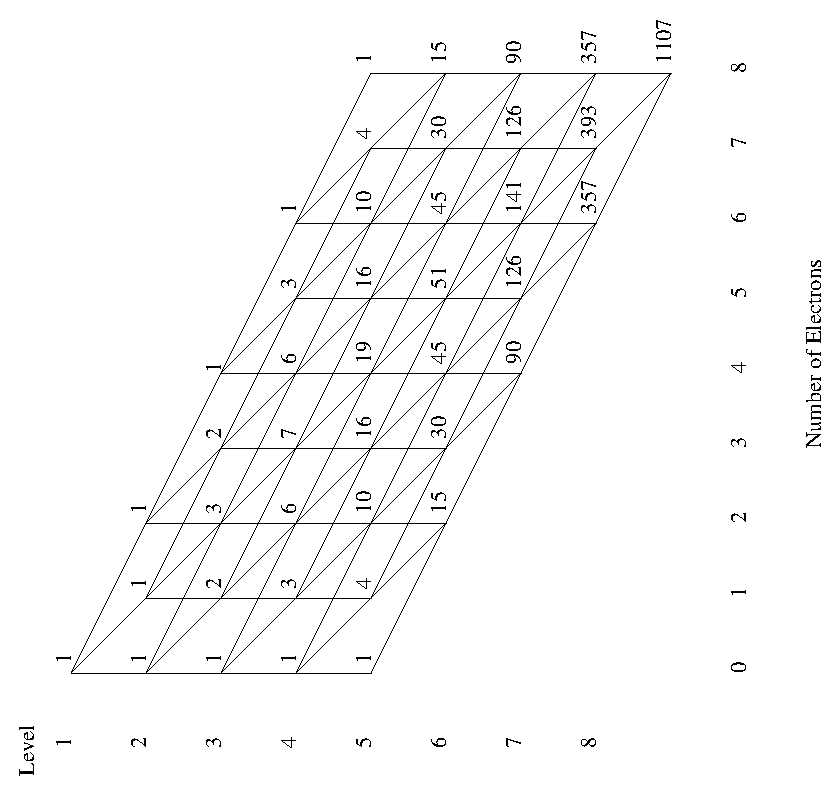
\includegraphics[angle=270]{orbitalgraph.eps}
\caption{\label{ograph} Orbital occupation graph for a full-CI with 8
electrons in eight orbitals.}
\end{figure}

\begin{table}[htbp]

\center

\begin{tabular}{lc|lc}
  Index  & Walk  & Index & Walk \\ \hline
   1 & 2 2 2 2 0 0 0 0   &1084 & 0 0 2 0 1 1 2 2 \\
   2 & 2 2 2 1 1 0 0 0   &1085 & 1 0 0 1 1 1 2 2 \\
   3 & 2 2 1 2 1 0 0 0   &1086 & 0 1 0 1 1 1 2 2 \\
   4 & 2 1 2 2 1 0 0 0   &1087 & 0 0 1 1 1 1 2 2 \\
   5 & 1 2 2 2 1 0 0 0   &1088 & 0 0 0 2 1 1 2 2 \\
   6 & 2 2 2 0 2 0 0 0   &1089 & 1 0 0 0 2 1 2 2 \\
   7 & 2 2 1 1 2 0 0 0   &1090 & 0 1 0 0 2 1 2 2 \\
   8 & 2 1 2 1 2 0 0 0   &1091 & 0 0 1 0 2 1 2 2 \\
   9 & 1 2 2 1 2 0 0 0   &1092 & 0 0 0 1 2 1 2 2 \\
  10 & 2 2 0 2 2 0 0 0   &1093 & 2 0 0 0 0 2 2 2 \\
  11 & 2 1 1 2 2 0 0 0   &1094 & 1 1 0 0 0 2 2 2 \\
  12 & 1 2 1 2 2 0 0 0   &1095 & 0 2 0 0 0 2 2 2 \\
  13 & 2 0 2 2 2 0 0 0   &1096 & 1 0 1 0 0 2 2 2 \\
  14 & 1 1 2 2 2 0 0 0   &1097 & 0 1 1 0 0 2 2 2 \\
  15 & 0 2 2 2 2 0 0 0   &1098 & 0 0 2 0 0 2 2 2 \\
  16 & 2 2 2 1 0 1 0 0   &1099 & 1 0 0 1 0 2 2 2 \\
  17 & 2 2 1 2 0 1 0 0   &1100 & 0 1 0 1 0 2 2 2 \\
  18 & 2 1 2 2 0 1 0 0   &1101 & 0 0 1 1 0 2 2 2 \\
  19 & 1 2 2 2 0 1 0 0   &1102 & 0 0 0 2 0 2 2 2 \\
  20 & 2 2 2 0 1 1 0 0   &1103 & 1 0 0 0 1 2 2 2 \\
  21 & 2 2 1 1 1 1 0 0   &1104 & 0 1 0 0 1 2 2 2 \\
  22 & 2 1 2 1 1 1 0 0   &1105 & 0 0 1 0 1 2 2 2 \\
  23 & 1 2 2 1 1 1 0 0   &1106 & 0 0 0 1 1 2 2 2 \\
  24 & 2 2 0 2 1 1 0 0   &1107 & 0 0 0 0 2 2 2 2 \\ \hline
\end{tabular}

\caption{\label{owalks} The first and last twenty-four lexically
ordered walks on an 8-electron 8-orbital full-CI orbital occupation graph.}
\end{table}

Spatial symmetry is in the code in a rudimentary, but useful, fashion.
The walks are ordered as if there is no symmetry (c.f., Table
\ref{owalks}) and the symmetry of each walk is simply computed as the
direct product of the symmetry of the singly-occupied orbitals
(directly available from the routine \verb!fci_owalk_info()!, Section
\ref{sec:fciowalkinfo}).  Only walks/occupations of the desired
symmetry are included in the CI vector (Section \ref{sec:ciindex}).
This facilitates use of symmetry to reduce the storage required for
the CI vector, and also the computation of matrix elements for
perturbation methods.  It also makes it easy to use the routines in
instances when you want to sum over all intermediate states regardless
of symmetry.  However, the walks of a specific symmetry are not
grouped together and symmetry is not presently used to reduce the
expense of the CI eigenvalue problem.

An alternative approach, which I've used in other programs,
is to modify the orbital graph by splitting each node so
that there is one for each irreducible representation.  The symmetry
of an orbital must be taken into account when singly occupying it so
that the node of the correct occupation and symmetry is connected to
on the next level.  This was, I think, first introduced by Shavitt
\cite{shavittguga,shavittguga2} in the 4-way graph (or distinct row
table, DRT) of the graphical unitary group approach (GUGA).

\section{Indexing the CI vector}
\label{sec:ciindex}

The CI vector looks like a two-dimensional array, $C_{\nu I}$ with the
outermost index running over orbital occupations ($I$) in lexical
order, and the innermost index ($\nu$) over possible spin functions
for that orbital occupation, again in lexical order.  Since the number
of spin functions varies with the number of singly occupied orbitals
in $I$, the CI vector is stored as a one-dimensional vector with an
index vector of dimension the number of orbital walks to point to the
beginning of the coefficients for a given walk $I$ (see the routine
\verb!fci_owalk_info()!, Section \ref{sec:fciowalkinfo}).  Note that
only coefficients of the correct symmetry are stored and therefore the
index into the CI vector is only meaningful for these orbital walks
and care must be taken to ensure the correct symmetry before trying to
use an index into the CI vector.

An interesting variation would be to group together within the CI
vector all orbital occupations with the same number of singly-occupied
orbitals.  Within each group the number of spin functions is now the
same and the CI vector may be treated as a two-dimensional array.

\section{More details on the graphical representations}

\subsection{Primitive spin graphs}

Primitive spin graphs are slightly easier since they have at most two
arcs from any node.  Nodes are labelled by the number of singly
occupied orbitals ($s$) and the intermediate $S_z=m$.  The weight of a
node $d(s,m)=d^s_m$ is then
\begin{equation}
 d^s_m = d^{s-1}_{m-\half} + d^{s-1}_{m+\half} \mbox{\ with\ } d^0_0 =
1 \label{spinnodeweight}
\end{equation}
in which nodes with no connecting arcs have zero weight.
The lexical ordering of walks on a graph is established by assigning a
weight to each arc on the graph.  The arcs weights are labelled as
follows
\begin{eqnarray}
 Y^{s-}_m & \mbox{connects} & (s,m) \rightarrow (s+1,m-\half ) \\
 Y^{s+}_m & \mbox{connects} & (s,m) \rightarrow (s+1,m+\half )
\end{eqnarray}

\begin{figure}[htbp]

\center

%\centerline{\psfig{figure=spinarcs.eps,angle=270}}
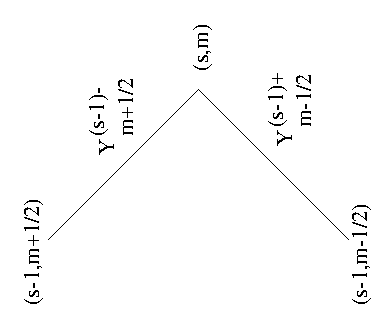
\includegraphics[angle=270]{spinarcs.eps}
\caption{\label{spinarcs} The two arcs coming into node $(s,m)$ on a
primtive spin graph, and their arc weights.}
\end{figure}
  
 The weight ($w_{\sigma}$) or lexical index of a walk
($\{\sigma_j:j=1,s\}$, c.f., Table \ref{mwalks}) is just
\begin{equation}
 w_{\sigma} = 1 + \sum_{j=1}^{s} Y_{m_j}^{s_j \sigma_j} \label{spinwalkweight}
\end{equation}
where $s_j$ and $m_j$ are the intermediate values of the number of
electrons and $S_z$ at nodes along the walk. 

An arc is assigned a weight equal to the number of walks from
the current node that have lower index.  The standard lexical ordering
corresponds to walking from right to left with the upward arc (right
to left!) being of lower index.  Thus, considering the two arcs going
from right to left from node $(s,m)$ 
(see Figure \ref{spinarcs}) the lexical ordering is
accomplished by the following assignments
\begin{eqnarray}
  Y^{(s-1)-}_{m+\half} & = & 0 \nonumber \\ 
  Y^{s+}_m & = & d_{s-1}^{m+\half}  \label{spinarcweights}
\end{eqnarray}
For computational convenience, an arc that does not exist is assigned
zero weight.  There is no need for a primtive (or spin-adapted) spin
graph to have separate node and arc weight tables, however, the
current code does do this.  They are small so the additional memory is
not an issue.

\subsection{Orbital graphs}

Nodes on an orbital graph are labelled by the level ($l$), which
corresponds the orbital being occupied by arcs going down, and the
number of electrons $n$.  When spatial symmetry is introduced there
will be an additional index for each irreducible representation.  The
weight ($k^l_n = k(l,n)$) of each node is simply
\begin{equation}
  k^l_n = k^{l-1}_{n-2} + k^{l-1}_{n-1} + k^{l-1}_n \label{orbnodeweight}
\end{equation}
where it is assumed that nodes with no connecting arcs have zero weight.

\begin{figure}[htbp]

\center

%\centerline{\psfig{figure=orbitalarcs.eps,angle=270}}
\includegraphics[angle=270]{orbitalarcs.eps}
\caption{\label{orbitalarcs} The three arcs, and their weights,
coming into node $(l,n)$ on an orbital occupation graph.}
\end{figure}

The three possible arcs descending from a node are (see Figure
\ref{orbitalarcs})
\begin{eqnarray}
 Z^{l,0}_{n} & \mbox{connects} & (l,n) \rightarrow (l+1,n) \\
 Z^{l,1}_{n} & \mbox{connects} & (l,n) \rightarrow (l+1,n+1) \\
 Z^{l,2}_{n} & \mbox{connects} & (l,n) \rightarrow (l+1,n+2)
\end{eqnarray}
and again the weight ($w_z$) of an orbital walk ($\{z: z_l,l=1,M\}$, for
$M$ orbitals, $z_l=0,1,2$) or occupation pattern, is simply
\begin{equation}
  w_z = 1 + \sum_{l=1}^{M} Z^{l,z_l}_{n_l} \label{orbwalkweight}
\end{equation}
where $n_l$ is the intermediate number of electrons at each node in
the walk.  Note that in the full-CI program the arcs $Z^{l,j}_n,
j=0,1,2$ are actually indexed with $j=1,2,3$ for historical reasons.

The lexical ordering of orbital walks is such that in traversing the
graph from bottom to top walks the rightmost arcs have lowest lexical
weight (the first and last twenty four walks on the graph in Figure
\ref{orbitalgraph} are given in Table \ref{owalks}).
Thus, the weight of an upward bound arc should be equal to the number
of possible walks that traverse other arcs from the same node that are
to the right of the arc of interest.  Considering again the three arcs
going up from node $(l,n)$ (Figure \ref{orbitalarcs}) 
\begin{equation}
  Z^{l-1,j}_{n-j} = Z^{l-1,j-1}_{n-j+1} + k^{l-1}_{n-j+1} \mbox{\ with\ }
  Z^{l-1,0}_n = 0 \label{orbarcweights}
\end{equation}
where $k^{l-1}_{n-j+1}$ (Equation \ref{orbnodeweight}) is the number of
walks coming down from node $(l-1,n-j+1)$.  Again, for computational
convenience, arcs and nodes that do not exist are assigned zero
weight. 

Aside: Multiple tails can be accomodated on the same graph by setting
the weight of $Z^{M,0}_n$ to be the sum of the weights of other tails
to the right.

\subsection{Constructing the weights and walking the graphs}

The node weights are readily formed by traversing the graphs from head
to tail (left to right for the spin graphs, top to bottom for the
orbital graphs) using the recursive formulae for the node weights
(Equations \ref{orbnodeweight} and \ref{spinnodeweight}). 

The arc weights are then determined by traversing the graphs from tail
to head (right to left for the spin graphs, bottom to top for the
orbital graphs) using the recursive formulae for the arc weights
(Equations \ref{spinarcweights} and \ref{orbarcweights}).

Given a walk on a graph (i.e., either a spin or orbital occupation
pattern) the lexical weight is readily computed from the arc weights
(Equations \ref{spinwalkweight} and \ref{orbwalkweight}). This
requires $O(N)$ array references and integer additions (where $N$ is
the number of open shells or the number of orbitals for spin and
orbital graphs respectively).

Determining the occcupation from the lexical weight is only slightly
harder.  Starting from the tail of the graph we accumulate the weight
of a trial walk (initialized to 1), and at each node we take the
highest weight arc (i.e., the lowest spin arc, or the leftmost orbital
arc) that is consistent with the incremented walk weight being less
than or equal to the weight of the walk we are seeking.  This process
requires $O(N)$ comparisons as well as $O(N)$ array look-ups and
integer additions.

\section{Matrix elements of orbital replacement operators}

In the determinant basis it is easy to compute matrix elements of
spin-dependent operators, however, I presently restrict attention to
spin-adapted operators (e.g., $E_{ij}$) which act as spatial orbital
replacement operators.  By doing this the formalism for evaluating
matrix elements over both CSF and determinants is exactly the same (I
think it can be made the same even in the case of spin-dependent
operators but only with an extended notation).

\begin{enumerate}
\item Note that an orbital replacement operator commutes with
permutations that act on the electrons --- the labels are independent.

\item Let $\hat{Q}$ be an orbital replacement operator and let $|K\! >$
and $|I\! >$ be orbital configurations in standard order (Section
\ref{standardorder}) such that
\begin{eqnarray}
  |K\! > & = & Q |K^Q\! > =  Q \hat{Q} |I\! > \mbox{, or}
\label{qik1} \\
  \hat{Q} \; |I \! > & = & Q^{-1} |K \! > \label{qik}
\end{eqnarray}
where $|K^Q\! >$ is an orbital configuration in {\em non-standard}
order that is produced by the action of $\hat{Q}$ on $|I\! >$.  $Q$ is
the electronic permutation that returns $|K^Q\! >$ to standard
occupation order.  This is the line-up permutation (or the inverse of
it depending on your perspective).

\item Recall that a determinant or CSF is written 
\begin{equation}
|I \lambda\! > = {\cal A} \; |I\! > \Theta_{\lambda} \label{csfdefn}
\end{equation}

\item Also recall these properties of the antisymmetrizer
\begin{eqnarray}
 {\cal A} & = & \frac{1}{\sqrt{n!}} \sum_P (-1)^P P \\
          & = & {\cal A}^{\dagger} \\
 {\cal A}^2 & = & \sqrt{n!} {\cal A} \\
     PA & = & AP = (-1)^P A \label{paap}
\end{eqnarray}

\item The action of $\hat{Q}$ on a determinant or CSF is then formed
as follows
\begin{eqnarray}
  \hat{Q} |I \lambda\! > 
  & = & \hat{Q} \; {\cal A} \; |I\! > \Theta_{\lambda} \mbox{, defined
by \ref{csfdefn}} \\
  & = & {\cal A} \; \hat{Q} \; |I\! > \Theta_{\lambda} \mbox{, from
independence of orbital and electronic labels} \\
  & = & {\cal A} \; \left( \hat{Q} \; |I\! > \right) \Theta_{\lambda}
\mbox{, since only I contains orbital labels} \\
  & = & {\cal A} \; \left( Q^{-1} \; |K\! > \right) \Theta_{\lambda} 
\mbox{, using \ref{qik}} \\
  & = & \left[ {\cal A} \; (-1)^Q Q \right]  \left( Q^{-1} \; |K\! >
\right) \Theta_{\lambda} \mbox{, using \ref{paap}} \\
  & = & {\cal A} \; (- 1)^Q |K\! > \left( Q \; \Theta_{\lambda} \right) 
 \\
  & = & {\cal A} \; |K\! > \left(  (- 1)^Q  \sum_{\mu} \Theta_{\mu}
U_{\mu \lambda}(Q) \right)  \\
  & = & (-1)^Q \sum_{\mu} |K \mu\! > U_{\mu \lambda}(Q)
\end{eqnarray}
where $U_{\mu \lambda}(Q)$ is an element of the representation matrix
of the permutation $Q$ in the spin-function basis.  The phase-factor
may also be included in $U$ in which case it is referred to as the
contra-gradient representation.

\item Using the above results we can readily obtain the value for the
matrix element
\begin{eqnarray}
 <\! K\nu | \hat{Q} | I \lambda\! > & = & (-1)^Q \sum_{\mu}
  <\! K \nu | K \mu \! > U_{\mu \lambda}(Q) \label{lineupeqn} \\
  & = & (-1)^Q U_{\nu \lambda}(Q) 
\end{eqnarray}
In Equation \ref{lineupeqn} only one term survives because of the
orthogonality of the spatial orbitals and the chosen spin function
bases (both primitive and spin adapted).
\end{enumerate}

What line-up permutations ($Q$) are of interest?  Consider $\hat{Q} =
E_{ij}$ where orbital $j$ is singly occupied in $|I\! >$ ($n_j^I = 0$)
and orbital $i$ is unoccupied ($n_i^I=0$).  This simply replaces
orbital label $j$ with $i$.  Let $\overline{i}$ and $\overline{j}$ be
the correct standard position of orbitals $i$ and $j$ respectively
amoung the singly occupied orbitals (which should be occupied in
increasing order).  Furthermore, let us assume that $i < j$.  Then,
the permutation of the (singly occupied) electronic coordinates that
restores the correct ordering of the occupation is the cyclic
permutation $(\overline{i} \ldots \overline{j})$.  The situation for
$j$ doubly occupied, or $i$ singly occupied is similar, but we defer
discussion of this since additional simplifications are possible.

A detailed example may help. Considering just the singly occupied
orbitals and with
\begin{equation}
 |I \! > = \phi_1(1) \phi_3(2) \phi_4(3) \phi_5(4) \phi_6(5)
\end{equation}
then, we see that 
\begin{eqnarray}
  E_{25} |I \! >  & = & \phi_1(1) \phi_3(2) \phi_4(3) \phi_2(4)
\phi_6(6) \\
 & = & \phi_1(1) \phi_2(4) \phi_3(2) \phi_4(3) \phi_6(5) 
\end{eqnarray}
(which is denoted $K^Q$ in Equation \ref{qik1}).  But the standard
order of occupation should be
\begin{equation}
  |K \! >  =  \phi_1(1) \phi_2(2) \phi_3(3) \phi_4(4) \phi_6(5)
\end{equation}
and the permutation of the {\em electronic} labels that accomplishes
this is the cyclic permutation $(2 3 4) = (2 3)(3 4)$.  This maps
electron 2 into electron 3, electron 3 into electron 4, and electron 4
back into electron 2.
\begin{equation}
  (2 3 4) \left[ \phi_1(1) \phi_2(4) \phi_3(2) \phi_4(3) \phi_6(5) 
\right] = \phi_1(1) \phi_2(2) \phi_3(3) \phi_4(4) \phi_6(5)
\end{equation}
The correct position of orbital 5 amoung the singly occupied orbitals
in $I$ is $\overline{j}=4$ and that of orbital 2 is $\overline{i}=2$.

\subsection{Computing matrix elements}

In the primitive spin or determinant basis, there will be just one
non-zero element in each row or column of the representation matrix
($U_{\mu \lambda}(Q)$) for any permutation, whereas the representation
matrices for spin adpated bases will be rather dense.  This fact may
be exploited (Duch \cite{duchspinad}) by just storing, in what Duch
named Primitive Spin Function Transformation Tables, the index to which
each primitive spin function transforms under the action of all cyclic
permutations and the corresponding phase factor.

For small FCI calculations this is very effective and it is what was
implemented in the original code. However, larger calculations have
too much data to hold since the number of entries is $5*(s+1)^2d^s_m$
which becomes very large for more than 10 or 12 active orbitals (the
factor of 5 arises from the various occupation cases).  Duch
recommended various alternatives, but following Knowles and Werner
\cite{knowleseai}, and in the spirit of the $N-2$ particle subspace
projection of Zarrabian et al \cite{zarrabian,harrison}, we can use the
following factorization
\begin{equation}
 E_{ij} = E_{ia}E_{aj}
\end{equation}
where $a$ is a ficticious orbital of index higher than any other
orbital.  This is equivalent to factorizing the cyclic permutation as 
\begin{equation}
(\overline{i} \ldots \overline{j}) = (\overline{i} \ldots s)(s \ldots
\overline{j}) \mbox{\ for\ } i < j
\end{equation}
where, again, $s$ is the number of open shell electrons.  It is also
akin to the action of an annihilation operator but rather than keeping
track of the $s-1$ electron states we just put the electron into a
fictitious orbital.  With this factorization there are only two
occupation cases to consider (with a total of three entries) since $a$
is always empty and there is a total of only $3(s+1)d^s_m$ entries to
be stored which is tractable for very large numbers of open shells.

The code constructs just the transformations associated with $<\!
K\mu|Eaj|J\nu\! >$ for $n_j=1,2$.  This is done as follows, initially
for $n_j = 1$.
\begin{enumerate}
\item Loop thru primitive spin functions $\nu$ for $s$ open shell
electrons and obtain the corresponding occupation pattern (by calling
\verb!fci_find_mocc!).

\item Loop thru $j=1,s$ corresponding to the cycles $(s \ldots j)$ for
$j=1,s$ and apply it to the occputation pattern.

\item Determine the lexical index of the generated occupation (by
calling \verb!fci_find_mweight!).  Store this multiplied by the parity
of the permutation in $T(\nu,j,1)$.
\end{enumerate}

For $n_j=2$ the situation is only slightly more complex since we will
obtain two $s+2$ electron occupations from breaking the alpha--beta pair.
\begin{enumerate}
\item Loop thru primitive spin functions $\nu$ for $s$ open shell
electrons, and obtain the corresponding occupation pattern (by calling
\verb!fci_find_mocc!).

\item Loop thru $j=1,s+1$ corresponding to the position amoung the
singly occupied orbitals of the new orbital.

\item First excite the alpha spin electron by constructing an $s+2$
electron spin function by appending ``\verb!+!'' to the $s$ electron
spin function $\nu$ and inserting a ``\verb!-!'' immediately before
position $j$.  Determine the new $s+2$ lexical walk index and store
it times the phase of the permutatation (the parity of $(j \ldots
1)(s+2 \ldots 1)$ is $(-1)^{s+j}$) in $T^{s,2}_{\nu,j}$.

\item Next excite the beta spin electron by constructing an $s+2$
electron spin function by appending ``\verb!-!'' to the $s$ electron
spin function $\nu$ and inserting a ``\verb!+!'' immediately before
position $j$.  Determine the new $s+2$ electron walk index and store
it with the negative of the previous parity (since we swapped the
first two electrons and the actual permutation is $(j \ldots
1)(s+2 \ldots 1)(1 2)$) in $T^{s,3}_{\nu,j}$.
\end{enumerate}

Finally, some logic is eliminated from the inner loop if instead of
storing the phase directly in the table as recommended by Duch
\cite{duchspinad}, we store it separately.  This does not require a
lot of memory since it is independent of the spin function index.  

\section{Density matrix operators}

Arbitrary-rank density matrix operators are very readily constructed
from the $E_{ai}$ operators \cite{knowleseai} since
\begin{equation}
 E_{pq,rs,tu,\ldots} =
E_{pa}E_{rb}E_{tc}\ldots E_{cu}E_{bs}E_{aq}
\end{equation}
where the fictitious orbitals are regarded as being ordered
$\cdots>c>b>a$.  This looks very much like the standard normal ordered
form of the operator in terms of annihilation/creation operators.  In
applying this expression in practice the following factorization has
several important properties in a determinant basis (with implied
summation over the repeated indices)
\begin{equation}
 < \! J\nu |E_{pq,rs,tu,\ldots}| I \omega \! > = 
 < \! J\nu |E_{pa}E_{rb}E_{tc}\ldots |N\mu \! >
 < \! N\mu |\ldots E_{cu}E_{bs}E_{aq}|I\omega \! > \\
\end{equation}
\begin{enumerate}
\item If the operators $E_{aq}$ etc. act only on open-shell electrons
then the number of open-shell electrons is unchanged, and the mapping
from $\omega$ to $\mu$ is  one-to-one and dense (a permutation).
\item If the operators $E_{aq}$ etc. break a spin pair then the number
of electrons is increased by two and the mapping from $\omega$ to
$\mu$ is one-to-two.  There is some sparsity (less than 50\% for
singlets) in the increased space since some spin couplings cannot be
generated from the broken spin pair. For instance, examination of
Figure \ref{mgraph} shows that six open-shell electrons give rise to
20 determinants, which if a closed-shell spin pair is broken, can only
give rise to 40 determinants.  However, there are 70 determinants for
8 open shells.
\end{enumerate}

The coupling coefficient generation routines then work in a very
straightforward fashion, working from the outside to the middle, and
then multiplying the two halves together.  Each application of an
operator ($E_{aq}$) results in a mapping from the spin functions in
the input (ket) to those in the output (bra) indices and some
associated phases.  These are specified by the occupation of the
orbital that is having an electron removed ($q$ in this instance), and
by the position of this orbital in the standard ordering of singly
occupied orbitals (if this is orbital $q$ its position amoung the
singly occupied is referred to as $\overline{q}$ or \verb!qbar!).  So
some book keeping is necessary to keep track of this information.  The
routines are heavily commented and coded in a stylized fashion so they
should be self-explanatory.

\section{Application Program Interface --- API}

The following routines will be augmented so that they provide access
to all of the necessary information to compute matrix elements,
manipulate walks on the orbital and spin graphs, and convert between
determinant and CSF bases. 

Obviously, an application that needs FCI information in its innermost
loop may need to access that information directly from the FCI common
blocks for reason of efficiency.  However, since the common blocks
will need to change in order to accomodate orbital symmetry and
modification of the algorithm to compute the coupling coefficients, it
is strongly recommended that the API be used (or extended) wherever
possible.

\subsection{Setting-up and solving a full-CI}

\subsubsection{{\tt fci\_setup}}

\begin{verbatim}
  subroutine fci_setup(multiplicity, nactive, nelectrons,
 &     orbsyms, symstate,
 &     norbitalconfig, ndeterminants, nconfigurations,
 &     norbconfignosym)
  integer multiplicity      ! [input] Spin multiplicity
  integer nactive           ! [input] No. of active orbitals
  integer nelectrons        ! [input] No. of active electrons
  integer orbsyms(nactive)  ! [input] Symmetry of orbitals (1...8)
  integer symstate          ! [input] Desired symmetry of state
  integer norbitalconfig    ! [output] No. of orb. conf. WITH symmetry
  integer ndeterminants     ! [output] No. of determinants in FCI
  integer nconfigurations   ! [output] No. of configurations in FCI
  integer norbconfignosym   ! [output] No. of orb. conf. WITHOUT symmetry
\end{verbatim}
This routine must be called before anythine else to initialize the
internal FCI data structures.  The determinant CI vector using
symmetry will be of length \verb!ndeterminants! (equivalent to
\verb!nconfigurations! CSF).

\subsubsection{{\tt fci\_solve}}
\label{sec:fcisolve}
\begin{verbatim}
   subroutine fci_solvenew(nroot, thresh, maxvec, ecore, h, g, 
  &     work, lenwrk, roots, evecfilename, diagfilename)
   integer nroot             ! [input] No. of roots to find
   double precision thresh   ! [input] Threshold for residual norm
   integer maxvec            ! [input] Davidson subspace dim PER ROOT
   double precision ecore    ! [input] Nuclear repulsion+frozen core
   double precision h(nacttr) ! [input] h(ij) = h_{ij}
   double precision g(nacttr,nacttr) ! [input] g(ij,kl) = (ij|kl)
   integer lenwrk            ! [input] Size of work space
   double precision work(lenwrk) ! [scratch] Work space
   double precision roots(nroot) ! [output] Returns the eigenvalues
   character*(*) evecfilename  ! [input] Name of file for eigen vectors
   character*(*) diagfilename  ! [input] Name of file for diagonals
\end{verbatim}

Solve the CI to the requested accuracy.  Currently uses determinants
but is readily extended to also accomodate CSF.  The eigenvalues are
returned in \verb!roots!.  The eigenvectors are returned in file
\verb!evecfilename!, and the diagonal elements of the Hamiltonian are
returned in \verb!diagfilename!.  The eigenvectors and diagonal
elements may be read using the routine \verb!fci_readvectors()!
(Section \ref{sec:fcireadvectors}).

The input integrals are stored as
\verb!h(ij)!=$h_{ij}$ and \verb!g(ij,kl)!=$(ij|kl)$, with $i \geq j$,
$k \geq l$, \verb!ij!=$i(i-1)/2$, and \verb!kl!=$k(k-1)/2+l$.  Have a
look at \verb!fci_load.F! to see how an ASCII list of integrals are
read in an inserted into these arrays in the test program.

The minimum amount of workspace required (\verb!lenwrk!)is independent
of the number of roots, and must exceed 2*\verb!ndeterminants!.  The
more memory the better, but 2*\verb!ndeterminants!+500000 will
probably always be enough.

Also, there is currently no possibility of restart, and the lowest
diagonal guess is always used.

\subsubsection{{\tt fci\_readvectors}}
\label{sec:fcireadvectors}
\begin{verbatim}
  subroutine fci_readevectors(ndets, nvec, v, filename)
  integer ndets             ! [input] Vector length
  integer nvec             ! [input] No. 
  double precision v(ndets,nvec)
  character*(*) filename
\end{verbatim}

The FCI package uses word-addressable random access files that cannot
be accessed using standard Fortran I/O operations.  This routine
enables the eigen-vectors and diagonal elements to be read from disk
by specifying the appropriate filename after \verb!fci_solve()! has
sucessfully completed.  To read the eigenvectors, specify \verb!nvec!
as \verb!nroot!.  To read the diagonal elements, specify \verb!nvec!
as one.

\subsection{Inquiring about occupations and dimensions}

\subsubsection{{\tt fci\_ofind\_occ}}
\begin{verbatim}
   subroutine fci_ofind_occ(iwalk,iocc)
c  
c  find the orbital occupation of walk with lexical index iwalk
c     
   integer iwalk             ! [input]
   integer nel               ! [input]
   integer iocc(*)           ! [output]
\end{verbatim}

\subsubsection{{\tt fci\_ofind\_weight}}
\begin{verbatim}
   subroutine fci_ofind_weight(iwalk,iocc)
   implicit none
c     
c  find the lexical index of a path on the orbital graph
c     
   integer iwalk             ! [output]
   integer iocc(*)           ! [input]
\end{verbatim}

\subsubsection{{\tt fci\_mfind\_occ}}
\begin{verbatim}
   subroutine fci_mfind_occ(iwalk,iocc,ns)
c     
c  given the lexical index of a path on a primitive spin graph
c  for ns electrons and multi=2sz+1, return the spin occupation
c     
   integer iwalk             ! [input]
   integer iocc(*)           ! [output]
   integer ns                ! [input]
\end{verbatim}

\subsubsection{{\tt fci\_mfind\_weight}}

\begin{verbatim}
   subroutine fci_mfind_weight(iwalk,iocc,ns)
   implicit none
c     
c  find the lexical index of a path on a primitive spin graph
c  for ns electrons and multi=2sz+1, given the spin occupation
c     
   integer iwalk             ! [output]
   integer iocc(*)           ! [input]
   integer ns                ! [input]
\end{verbatim}

\subsubsection{{\tt fci\_num\_dets}}
\label{sec:fcinumdets}
\begin{verbatim}
   integer function fci_num_dets(ns)
c
c  return the number of determinants for ns open shell electrons
c  assuming that ns is a valid no. of open shell electrons for
c  the given FCI space and spin multiplicity
c
   integer ns                ! [input]
\end{verbatim}

\subsubsection{{\tt fci\_num\_csf}}
\begin{verbatim}
   integer function fci_num_dets(ns)
c
c  return the number of configurations for ns open shell electrons
c  assuming that ns is a valid no. of open shell electrons for
c  the given FCI space and spin multiplicity
c
   integer ns                ! [input]
\end{verbatim}

\subsubsection{{\tt fci\_num\_owalks}}
\begin{verbatim}
  integer function fci_num_owalks()
c
c Returns the number of orbital occupation walks in the FCI
c ignoring symmetry.
c
\end{verbatim}

\subsubsection{{\tt fci\_ndets}}
\begin{verbatim}
  integer function fci_ndets()
c
c Returns the total number of determinants in the FCI
c (with use of symmetry)
c
\end{verbatim}

\subsubsection{{\tt fci\_ncsf}}
\begin{verbatim}
  integer function fci_ncsf()
c
c Returns the total number of spin-adapted configurations in the FCI
c (with use of symmetry)
c
\end{verbatim}

\subsubsection{{\tt fci\_max\_num\_dets}}
\begin{verbatim}
  integer function fci_max_num_dets()
c
c Returns the maximum number of determinants associated
c with any orbital configuration in the full CI.
c
c [Note that occupations K that arise as a result of
c .factorizations such as <I|Eij|J>=<I|Eia|K><K|Eaj|J>
c .where a is a ficitious orbital, may have more open shells.  
c .However, these are only relevant in the internals of the 
c .coupling coefficient generation routines]
\end{verbatim}

\subsubsection{{\tt fci\_owalk\_info}}
\label{sec:fciowalkinfo}
\begin{verbatim}
  subroutine fci_owalk_info(owalk, iocc, ns, ioff, numdet, sym)
c     
c Given the index of an orbital walk return the occupation, the 
c offset in the CI determinant vector, the number of open shells,
c the corresponding number of determinants, and the symmetry of 
c the occupation.  
c  
c The CI coefficients for this orbital occupation are addressed
c as C(ioff+i) i=1,...,numdet.
c     
c This routine bundles the function of several other routines
c as a convenience.
c     
  integer owalk        ! [input]  Index of orbital occupation
  integer iocc(*)      ! [output] The orbital occupation pattern
  integer ns           ! [output] No. of open shells
  integer ioff         ! [output] Offset into CI vector
  integer numdet       ! [output] No. of determinants for this ns
  integer sym          ! [output] Symmetry 0...7
\end{verbatim}

\subsubsection{{\tt fci\_det\_to\_walk}}
\begin{verbatim}
   subroutine fci_det_to_walk(idet, owalk, mwalk)
c
c  Given the index of a determinant, idet, return the
c  corresponding lexical weights of orbital and primitive
c  spin functions.  Without having an index vector the
c  length of the CI expansion the only way to do this
c  is with a binary search, so this operation costs 
c  about log2(ndets).
c
   integer idet    ! [input] Index into determinant CI vector
   integer owalk   ! [output] Corresponding orbital index
   integer mwalk   ! [output] Corresponding primitive spin function index
\end{verbatim}

\subsection{Transforming between CSF and determinats, and spin adaption}

\subsubsection{{\tt fci\_spin\_adapt}}
\label{spinad1}
\begin{verbatim}
   subroutine fci_spin_adapt(ns, direction, det, csf)
c     
c  Given a set of coefficients of either determinants or CSF
c  corresponding to a single orbital occupation with ns open shells,
c  then do the following
c     
c  if (direction == 1)
c  ... project from determinants to CSF with multiplicity multi (fci_setup)
c  ... if there is spin contamination norm will not be conserved
c  else if (direction == 2)
c  ... project from CSF with multiplicity multi to determinants
c  ... norm should be conserved
c  else
c  ... invalid value for direction
c  endif
c     
   integer ns                ! [input] No. of open shells
   integer direction         ! [input] 1=det to csf, 2=csf to det
   double precision det(*)   ! [in/out] coefficients of determinants
   double precision csf(*)   ! [in/out] coefficients of csf
\end{verbatim}

The following related routine \verb!fci_spin_adapt_nvec()! can
transform multiple vectors (with the same number of open shells) at
once, which is much more efficient.

\subsubsection{{\tt fci\_spin\_adapt\_nvec}}
\begin{verbatim}
  subroutine fci_spin_adapt_nvec
 &     (ns, direction, det, ldd, csf, ldc, nvec)
c     
c Given NVEC sets of coefficients of either determinants or CSF
c corresponding to a single orbital occupation with ns open shells,
c then do the following
c   
c if (direction == 1)
c ... project from determinants to CSF with multiplicity multi (fci_init)
c ... if there is spin contamination norm will not be conserved
c else if (direction == 2)
c ... project from CSF with multiplicity multi to determinants
c ... norm should be conserved
c else
c ... invalid value for direction
c endif
c     
\end{verbatim}

\subsubsection{{\tt fci\_spin\_force}}
\begin{verbatim}
   subroutine fci_spin_force(c)
c  
c  Force determinant CI vector to be spin adapted by projecting
c  to and from the CSF space.  Also, renormalizes.
c     
   double precision c(ndets) ! [in/out] Determinant CI vector
\end{verbatim}

\subsection{Coupling coefficients}

\subsubsection{{\tt fci\_couple1}}

\begin{verbatim}
   subroutine fci_couple1(vec, nvec, p, iocc, idim, 
  &     numq, qlist, epq)
c  
c  Compute <V|Epq|Iw> for given CI vectors V, fixed 
c  orbital p, fixed orbital occupancy I (iocc), and all orbitals q
c  and primitive spin functions w.
c  
c  numq returns the number of orbitals q giving a nonzero interaction
c  
c  qlist(1...numq) contains the values of q
c  
c  epq(1...idim,1...nvec,1...numq) contains the coupling coeffcients
c  
   integer nvec              ! [input] No. of vectors on the left hand side
   double precision vec(ndets,nvec) ! [input] The CI vectors
   integer p                 ! [input] Fixed label on Epq
   integer iocc(nactiv)      ! [input] Orbital occupation of I
   integer idim              ! [input] No. of spin functions for I
   integer numq              ! [output] Returns the number of q
   integer qlist(*)          ! [output] Returns the list of interacting q
   double precision epq(idim,nvec,*) ! [output] epq(w,i,q) = <Vi|Epq|Iw>
\end{verbatim}
% & 

\subsubsection{{\tt fci\_couple2}}
\begin{verbatim}
   subroutine fci_couple2(vec, nvec, p, r, iocc, idim, 
  &     numqs, qslist, epqrs)
c  
c  Compute <V|Epq,rs|Iw> for given CI vectors V, fixed orbitals
c  p and r, fixed orbital occupancy I (iocc), and all orbitals q and s,
c  and primitive spin functions w.
c
c  The constraint (pq) >= (rs) is applied, so we loop over all q but
c  restrict the s loop.  If couple2 is called with p>=r then all unique
c  coeffs are generated.
c
c  numqs returns the number of orbitals q, s giving a nonzero interaction
c  
c  qslist(1, 1...numqs) contains the values of q
c  qslist(2, 1...numqs) contains the values of s
c  
c  epqrs(1...idim,1...nvec,1...numqs) contains the coupling coeffcients
c  
   integer nvec              ! [input] No. of vectors on the left hand side
   double precision vec(ndets,nvec) ! [input] The CI vectors
   integer p, r              ! [input] Fixed labels on Epq,rs
   integer iocc(nactiv)      ! [input] Orbital occupation of I
   integer idim              ! [input] No. of spin functions for I
   integer numqs             ! [output] Returns the number of q, s
   integer qslist(2,*)       ! [output] Returns the list of interacting q,s
   double precision epqrs(idim,nvec,*) ! [output] epq(w,i,q) = <Vi|Epqrs|Iw>
\end{verbatim}

\subsubsection{{\tt fci\_couple3}}
\begin{verbatim}
   subroutine fci_couple3(vec, nvec, p, q, r, t, iocc, idim, 
  &     numsu, sulist, epqrstu)
c  
c  Compute <V|Epq,rs,tu|Iw> for given CI vectors V, fixed orbitals
c  p,q,r,t and fixed orbital occupancy I (iocc), and all orbitals s,u
c  and primitive spin functions w.
c
c  Constrain the loops over s and u so that (pq)>=(rs)>=(tu).  If the
c  calling program externally constrains p>=r>=t (all q) then all
c  unique coupling coefficients will be generated.
c  
c  numsu returns the number of orbitals s,u giving a nonzero interaction
c  
c  sulist(1, 1...numsu) contains the values of s
c  sulist(2, 1...numsu) contains the values of u
c  
c  epqrstu(1...idim,1...nvec,1...numsu) contains the coupling coeffcients
c  
   integer nvec              ! [input] No. of vectors on the left hand side
   double precision vec(ndets,nvec) ! [input] The CI vectors
   integer p, q, r, t        ! [input] Fixed labels on Epq,rs,tu
   integer iocc(nactiv)      ! [input] Orbital occupation of I
   integer idim              ! [input] No. of spin functions for I
   integer numsu             ! [output] Returns the number of s,u
   integer sulist(2,*)       ! [output] Returns the list of interacting s,u
   double precision epqrstu(idim,nvec,*) ! [output] <Vi|Epqrstu|Iw>
\end{verbatim}


\subsection{Miscellaneous}

\subsubsection{{\tt fci\_onepdm}}
\begin{verbatim}
   subroutine fci_onepdm(vec, nvec, onepdm)
c  
c  Compute the 1-particle density matrices
c  
c  onepdm(p,q,ivec) returns <V(ivec)|Epq|V(ivec)>
c  
   integer nvec              ! [input] No. of vectors
   double precision vec(ndets, nvec) ! [input] The CI vectors
   double precision onepdm(nactiv,nactiv,nvec) ! [output] 1 PDMs
\end{verbatim}

The program checks the 1-PDMs for symmetry and the correct trace and
will abort if an error is detected.

The two-particle density matrix can also be generated with a small
modification to this routine.

\subsubsection{{\tt fci\_hv}}
\begin{verbatim}
  subroutine fci_hv(ecore, h, g, work, lenwrk, v, s)
c
c Compute the Hamiltonian matrix-vector product s = Hv 
c
  double precision ecore    ! [input] Frozen-core+nuclear replusion energy
  double precision h(nacttr) ! [input] Effective 1-e integrals Core+T+V
  double precision g(nacttr,nacttr) ! [input] Two-electron integrals
  integer lenwrk            ! [input] Size of workspace
  double precision work(lenwrk) ! [scratch] Workspace - the more the better
  double precision v(ndets) ! [input] CI vector
  double precision s(ndets) ! [output] s = H*v
\end{verbatim}

The Davidson diagonalizer calls this routine so it should be reliable.

\subsubsection{{\tt fci\_hami}}
\begin{verbatim}
   subroutine fci_hami(hamil, ecore, h, g, work, lenwork)
c
c  Simple wrapper routine to build the full triangular Hamiltonian
c  in the determinant basis from the one- and two-electron integrals
c
   double precision hamil(*) ! [output] Returns triangle of Hamiltonian
   double precision ecore    ! [input] Frozen core + nuclear replulsion
   double precision h(nacttr) ! [input] Triangle of 1-e integrals
   double precision g(nacttr,nacttr) ! [input] 2-e integrals
   integer lenwork           ! [input]
   double precision work(lenwork) ! [scratch]
\end{verbatim}

\subsubsection{{\tt fci\_diags}}
\begin{verbatim}
  subroutine fci_diags(hd,ecore,h,g,ionel,nonemx,kpt,mkpt)
c     
c     construct the diagonals of the hamiltonian 
c     
  double precision hd(ndets) ! [output] The diagonals
  double precision ecore    ! [input] Nuclear repulsion + frozen core
  double precision h(nacttr) ! [input] 1-e integrals
  double precision g(nacttr,nacttr) ! [input] 2-e integrals
  integer nonemx            ! [input] dimension of ionel
  integer ionel(5,nonemx)   ! [scratch] workspace for coupling coeff
  integer kpt(nonemx)       ! [scratch] workspace
  integer mkpt(ndetmx+1)    ! [scratch] workspace
\end{verbatim}
This is an internal interface to compute the diagonal elements on
demand.  It would be easy to provide an easy to use wrapper for this
(see usage in \verb!fci_solve.F!) but since \verb!fci_solve! (Section
\ref{sec:fcisolve}) already writes the diagonals to disk there is
not much point in using this routine elsewhere.

\subsubsection{{\tt fci\_prspnad}}
\begin{verbatim}
  subroutine fci_prspnad(ns)
  integer ns                ! [input]
c
c     Print the spin-adaption coefficents for ns open shells
c
\end{verbatim}

\subsubsection{{\tt fci\_tprint}}

\begin{verbatim}
  subroutine fci_tprint()
\end{verbatim}

This routine prints timing information to FORTRAN unit 6.  If a
routine is called more that $10^5$ times then to avoid too much system
call overhead the timing is automatically disabled and the time
reported as zero.  The number of calls is still accumulated.

\subsubsection{{\tt fci\_err}}
\begin{verbatim}
  subroutine fci_err(string, code)
  character*(*) string    ! [input]
  integer code            ! [input]
\end{verbatim}

All errors in the full-CI code are reported through this routine.
Put any additional error handling into this routine.

\begin{thebibliography}{99}
%\bibliographystyle{plain}
%\bibliography{xampl}

\addcontentsline{toc}{section}{References}

% \journal{label}{authors}{journal}{volume}{year}{page}

% \book{label}{authors}{title}{publisher}{year}

\bibitem{pauncz}{R. Pauncz}{Spin functions: Construction and use}{Plenum,
New York}{1979}

\bibitem{paunczsym}{R. Pauncz}{The Symmetric Group in Quantum
Chemistry}{CRC Press, Inc., Boca Raton, Florida, USA}{1995}

\bibitem{handyfci}{P. Saxe, D.J. Fox, H.F. Schaefer III and
N.C. Handy}{J. Chem. Phys.}{74}{1982}{5584}

\bibitem{knowleseai}{P.J. Knowles and H-J. Werner}{Chem. Phys. Lett.}{145}{1988}{514}

\bibitem{duchug}{W. Duch}{Int. J. Quant. Chem.}{27}{1985}{59}

\bibitem{duchspinad}{W. Duch}{Int. J. Quant. Chem.}{30}{1986}{799}

\bibitem{duchcouple}{W. Duch}{Chem. Phys. Lett.}{124}{1986}{442}

\bibitem{duchfci}{W. Duch}{Intern. J. Quant. Chem}{S24}{1990}{683}

\bibitem{duchsga}{W. Duch and
J. Karwowski}{Comp. Phys. Rep.}{2}{1985}{92}

\bibitem{paldusguga}{J. Paldus}{Phys. Rev. A}{14}{1976}{1620}

\bibitem{shavittguga}{I. Shavitt}{Int. J. Quant. Chem. Symp.}{11}{1977}{131}

\bibitem{shavittguga2}{I. Shavitt}{Int. J. Quant. Chem. Symp.}{12}{1978}{5}

\bibitem{saunders}V.R. Saunders and J.H. van Lenthe, Mol. Phys. 48, 1983 923.

\bibitem{zarrabian}{S. Zarrabian, C.R. Sarma and J. Paldus}{Chem. Phys. Lett.}{155}{1989}{183}

\bibitem{harrison}{R.J. Harrison and S. Zarrabian}{Chem. Phys. Lett.}{158}{1989}{393}

\bibitem{kotani}{M. Kotani, A. Amemiya, E. Ishiguro and T. Kimura}{Tables
of Molecular Integrals}{Maruzen, Co., Tokyo}{1955}

\end{thebibliography}

\end{document}


